 \section{引言}

近年来，深度学习与人工智能技术在自动驾驶系统中变得日益重要，这些系统需要在复杂驾驶场景中做出正确决策，以确保驾驶安全与舒适性。通常，自动驾驶系统包含多种任务，如检测、跟踪、在线建图、运动预测和规划。
如 \cref{fig:pipeline-a} 所示，传统模块化范式将复杂系统解耦为多个独立优化的单任务。在该范式中，独立的单任务模块之间存在手工设计的后处理环节，这使得整个流程变得更为臃肿。另一方面，由于堆叠任务间场景信息的有损压缩，整个系统的误差逐渐累积，可能导致潜在的安全问题 \cite{liang2020pnpnet, sadat2020perceive}。

针对上述问题，端到端（End-to-End）自动驾驶系统以更简洁的方式将原始传感器数据作为输入并直接返回规划结果。早期工作跳过中间任务，直接从原始传感器数据预测规划结果 \cite{codevilla2018end,codevilla2019exploring, wu2022trajectory, zhang2021end}。虽然这种方法更为直接，但在模型优化、可解释性和规划性能方面不尽如人意。另一种具有更好可解释性的多层面范式是将自动驾驶的多个部分整合到一个模块化的端到端模型中 \cite{hu2023planning, ye2023fusionad}，其中引入了多维监督以提高对复杂驾驶场景的理解，并带来多任务能力。

\begin{figure}[tb]
  \centering
  \begin{subfigure}{0.6\linewidth}
  \begin{subfigure}{1\linewidth}
    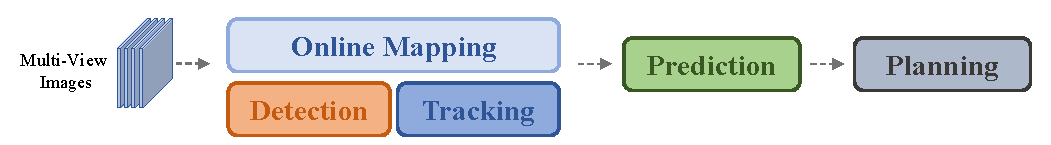
\includegraphics[width=1\linewidth]{Figures/Pipeline-a-Figure}
    \caption{传统自动驾驶范式}
    \label{fig:pipeline-a}
  \end{subfigure}
  \hfill
  \\
  \begin{subfigure}{1\linewidth}
    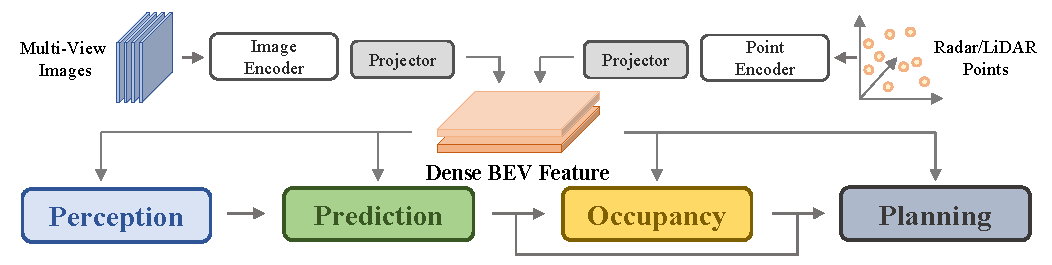
\includegraphics[width=1\linewidth]{Figures/Pipeline-b-Figure}
    \caption{密集BEV中心端到端范式}
    \label{fig:pipeline-b}
  \end{subfigure}
  \label{fig:short}
  \\
    \begin{subfigure}{1\linewidth}
    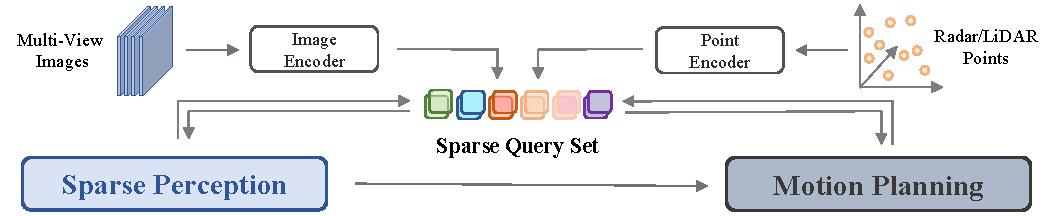
\includegraphics[width=1\linewidth]{Figures/Pipeline-c-Figure}
    \caption{稀疏查询中心端到端范式}
    \label{fig:pipeline-c}
  \end{subfigure}
  \hfill
  \end{subfigure}
  \begin{subfigure}{0.38\linewidth}
  \centering
    \begin{subfigure}{1\linewidth}
    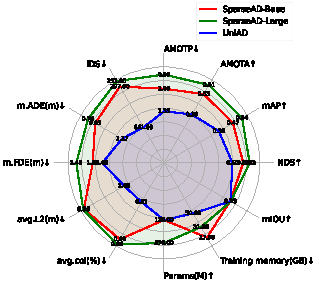
\includegraphics[width=1\linewidth]{Figures/RadarChart-Figure}
    \caption{本文方法与当前最优端到端自动驾驶方法\cite{hu2023planning}的综合性能对比}
    \label{fig:pipeline-d}
    \end{subfigure}
    \\
    \begin{subfigure}{1\linewidth}
    \end{subfigure}
    \\
    \begin{subfigure}{1\linewidth}
    \end{subfigure}

  \end{subfigure}

  \caption{主流自动驾驶范式对比。(a) 传统范式。(b) 密集BEV中心范式。(c) 本文提出的稀疏查询中心端到端自动驾驶范式。(d) (b)和(c)的代表性方法综合性能对比。}
  \label{fig:pipeline}
\end{figure}

如 \cref{fig:pipeline-b} 所示，在大多数先前的模块化端到端方法中，整个驾驶场景通过密集的鸟瞰视图（BEV, Bird's Eye View）特征表示，包括多传感器和时序信息，这些特征被用作包括感知、预测和规划在内的全栈驾驶任务的源输入。基于密集BEV特征在跨空间和时间的多模态和多任务中发挥关键作用这一事实，本文将先前采用BEV表示的端到端方法总结为\textbf{密集BEV中心（Dense BEV-Centric）}范式。
然而，尽管这些方法\cite{hu2023planning,ye2023fusionad}具有简洁性和可解释性，其在自动驾驶各子任务上的性能仍然远落后于相应的单任务方法 \cite{liu2022petr, wang2023exploring, pang2023standing, jiang2023vad}。此外，在密集BEV中心范式下，长时间时序融合和多模态融合主要通过多个BEV特征图实现，这带来了计算成本和内存占用的显著增加，给实际部署带来更多负担 \cite{zhang2023fully, jiang2023far3d}。

本文提出了一种新颖的\textbf{稀疏查询中心（Sparse Query-Centric）}范式用于端到端自动驾驶——SparseAD，其中整个驾驶场景中跨空间和时间的所有元素均由稀疏查询（Sparse Query）表示，无需任何密集BEV特征，如 \cref{fig:pipeline-c} 所示。借助稀疏表示，端到端模型能够更高效地利用更长的历史信息，并以显著更低的计算成本和内存占用扩展到更多模态和任务。

具体而言，本文改进了模块化端到端架构，将其简化为由稀疏感知（Sparse Perception）和运动规划器（Motion Planner）组成的简洁结构。在\textbf{稀疏感知}中，检测、跟踪和在线建图等感知任务通过通用时序解码器\cite{wang2023exploring}得到统一，其中多传感器特征和历史记忆被视为令牌（Token），目标查询（Object Query）和地图查询（Map Query）分别表示驾驶场景中的障碍物和道路元素。在\textbf{运动规划器}中，以稀疏感知查询作为环境表示，同时对自车和周围智能体进行多模态运动预测，为自车提供多种初始解决方案，然后综合考虑多个维度的驾驶约束以生成最终规划。值得注意的是，SparseAD卓越的效率使其能够通过先进的骨干网络 \cite{dosovitskiy2020image,liu2022convnet}、大规模预训练 \cite{fang2023eva,radford2021learning} 或海量数据来扩展模型规模以进一步提升性能。本文在流行的nuScenes数据集上进行了大量实验，验证了所提出的稀疏查询中心范式在端到端自动驾驶中的有效性和优越性，如 \cref{fig:pipeline-d} 所示。

总之，本文的主要贡献包括：
\begin{itemize}

\item 提出了一种新颖的\textbf{稀疏查询中心（Sparse Query-Centric）}范式用于端到端自动驾驶——\model，无需任何密集BEV表示，具有高效扩展到更多模态和任务的巨大潜力。

\item 将模块化端到端架构简化为稀疏感知和运动规划两部分，前者以完全稀疏的方式统一了检测、跟踪和在线建图，后者以更合理的框架实现运动预测和规划。

\item 在具有挑战性的nuScenes数据集\cite{caesar2020nuscenes}上，\model 在端到端方法中达到了SOTA性能，并显著缩小了端到端范式与单任务方法之间的性能差距，展示了所提出的稀疏端到端范式的巨大潜力。
\end{itemize}